
\section{Erkennung}

\begin{frame}[b]
	\begin{figure}
		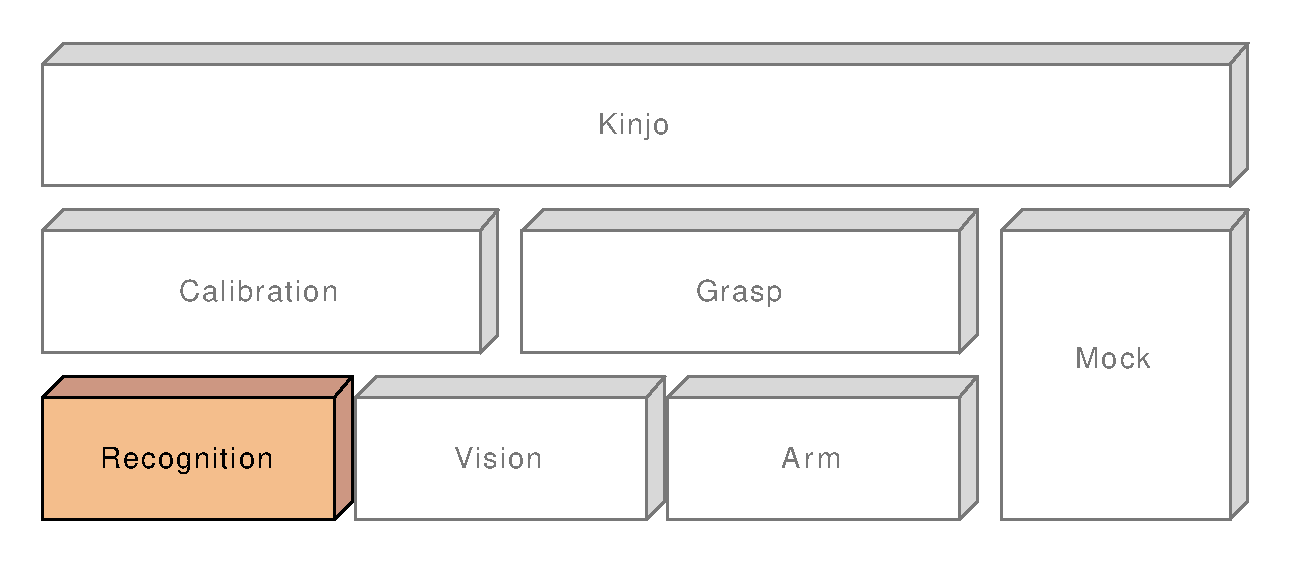
\includegraphics[width=0.8\textwidth]{nav_recognition}
	\end{figure}
	\vspace*{0.7cm}
\end{frame}

\begin{frame}[t]{Erkennung}
	\begin{itemize}
		\item Eingabe: RGB-Bild
		\item Ausgabe: XY-Pixel-Position und Radius des erkannten
			Kalibrierungsobjektes
		\item Aktuell nur für Kreisförmige Objekte beliebig einstellbarer
			Farbe
		\item Objekt bzw. Farbe muss eindeutig erkennbar sein
	\end{itemize}
\end{frame}

\begin{frame}[t]{Erkennung}
	\begin{block}{Abfolge}
		\begin{columns}[t]
			\begin{column}{0.4\textwidth}
				\only<1>{
					\begin{figure}
						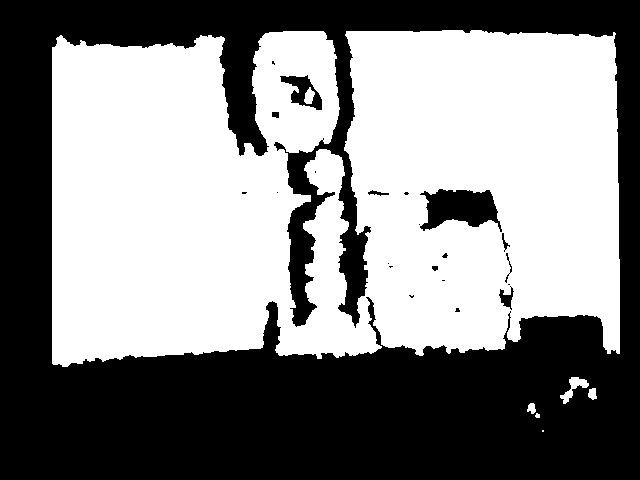
\includegraphics[width=\textwidth]{recognition_Depth}
					\end{figure}
				}
				\only<2-4>{
					\begin{enumerate}
						\item<2-4> Konvertierung von RGB- nach HSV-Farbraum (für einfacheres Maskieren des
							Farbbereiches in Schritt 2)
						\item<3-4> Maskieren der Pixel im erwarteten Farbbereich
						\item<4> Morphologische Operationen zum Entfernen von zu kleinen oder
							nicht kreisförmigen Strukturen
					\end{enumerate}
				}
				\only<5->{
					\begin{enumerate}
						\setcounter{enumi}{3}
						\item<5-> Blur für bessere Kreiserkennung
						\item<6-> Kreiserkennung mittels Hough-Transformation.
						\item<7-> Rating aller erkannten Objekte und Rückgabe des besten.
					\end{enumerate}
				}
			\end{column}
			\begin{column}{0.4\textwidth}
				\begin{figure}
					\includegraphics<1>[width=\textwidth]{recognition_RGB}
					\includegraphics<2>[width=\textwidth]{recognition_HSV}
					\includegraphics<3>[width=\textwidth]{recognition_Mask}
					\includegraphics<4>[width=\textwidth]{recognition_MaskFilter}
					\includegraphics<5>[width=\textwidth]{recognition_MaskFilterBlur}
					\includegraphics<6->[width=\textwidth]{recognition_RecognitionResult}
				\end{figure}
			\end{column}
		\end{columns}
	\end{block}
\end{frame}

